\section{\textit{Web App}}

(descrição capítulo)

\par \medskip

A aplicação \textit{web} é responsável por estabelecer uma interface sobre a qual as organizações podem interagir com a plataforma, disponibilizando às mesmas ferramentas que possibilitam a realização de operações como por exemplo a criação de \textit{posts} ou a realização de pesquisas sobre a plataforma.

\par \medskip

Foram definidos alguns requisitos chave no início da conceptualização da aplicação, como por exemplo:

\begin{itemize}
	\item disponibilizar meios para consultar os \textit{posts}, eventos e outros utilizadores da plataforma e interagir com os mesmos; 
	\item permitir às organizações editarem o seu perfil;
	\item possibilitar que as mesmas possam criar e editar \textit{posts} e eventos;
	\item apresentar contactos de voluntários interessados em eventos pertencentes à organização autenticada.
\end{itemize}

Numa fase inicial do projeto, foi considerada a opção de desenvolver a aplicação \textit{web} usando a \textit{framework} Angular.js. Contudo, após nova avaliação, optou-se por utilizar a tecnologia React. Esta alteração foi efetuada após verificar que React é a tecnologia mais usada no mercado à data da realização do projeto. 

\subsection{Utilização da web app}

Levando em consideração que este componente foi desenvolvido especificamente para organizações, a maioria das operações implicam que um utilizador organização esteja autenticado.

\begin{figure}[h]
	\centering
	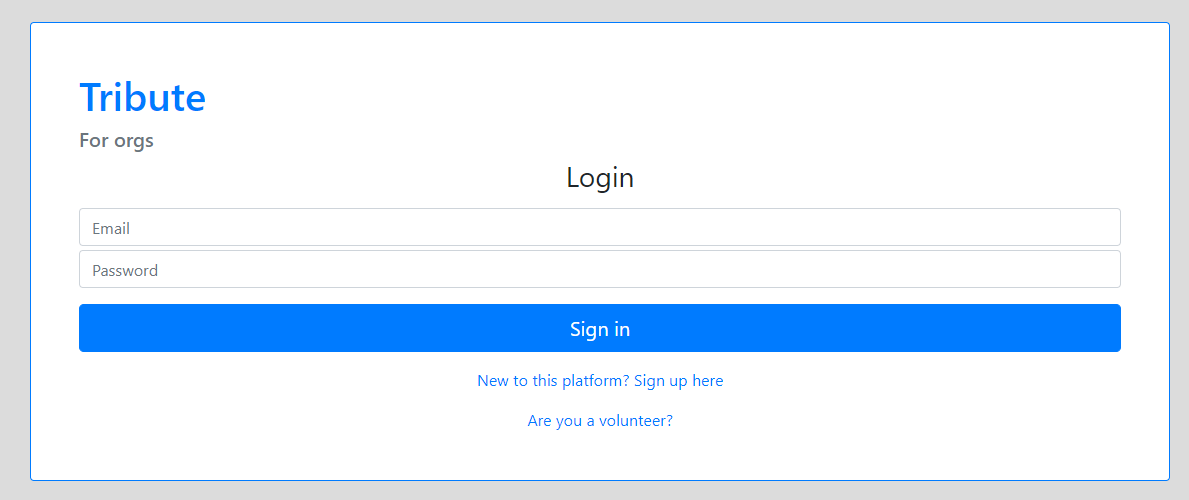
\includegraphics[scale=.38]{web_app_login_page}
	\caption{Interface de autenticação}
\end{figure}

Nesta versão da aplicação, é permitido que sejam registados utilizadores do tipo organização. Contudo, numa versão publicada da plataforma, o registo deste tipo de utilizadores seria realizado através do contacto direto dos mesmos com os gestores da aplicação de maneira a que apenas organizações fidedignas pudessem ter um perfil na plataforma.

\par \medskip

\begin{figure}[h]
	\centering
	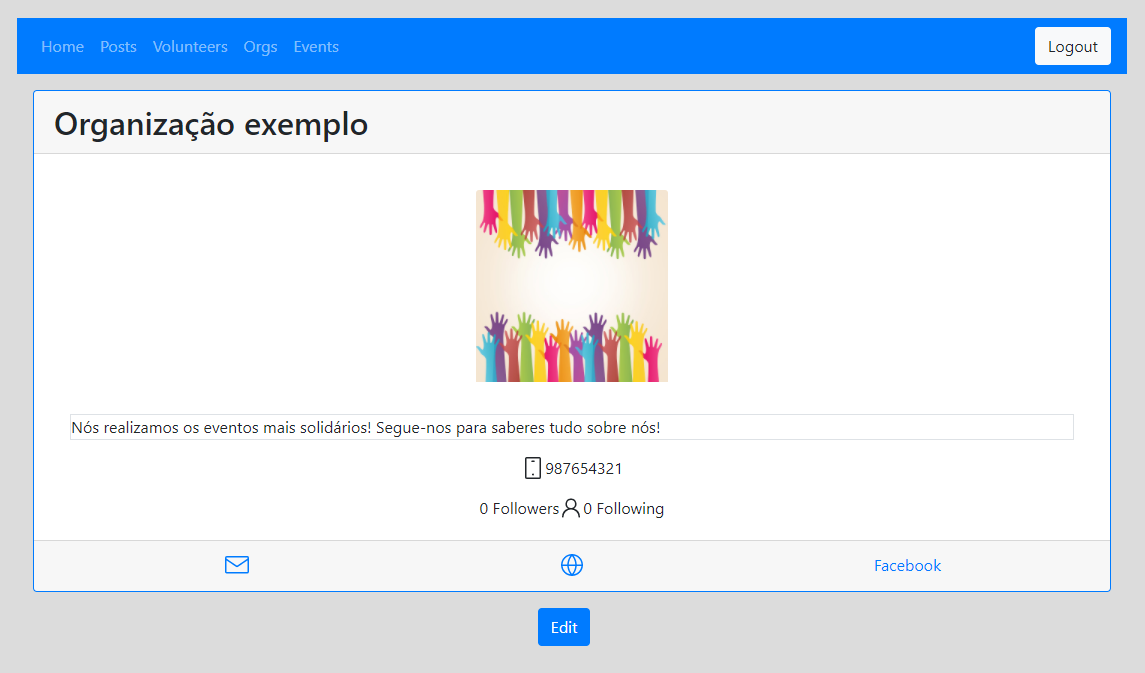
\includegraphics[scale=.38]{web_app_dashboard}
	\caption{Interface de autenticação}
\end{figure}

Após autenticação na aplicação, é disponibilizado um painel principal onde é possível navegar entre as várias páginas da aplicação e realizar as operações pretendidas.

\par \medskip

\subsection{Arquitetura}

A arquitetura da aplicação é composta principalmente por 2 módulos: API e Componentes e ainda a classe principal da aplicação.

\par \medskip 

Similar ao funcionamento do módulo com o mesmo nome na aplicação \textit{mobile}, API disponibiliza operações que realizam pedidos HTTPS à API. Componentes contém a implementação de todos os componentes \textit{react} apresentados ao utilizador, desde as páginas em si a componentes que são utilizados nestas. 

\par \medskip

A classe principal da aplicação é responsável não só por instanciar os serviços da API assim como definir o roteamento da aplicação \textit{web}.

\subsubsection{API}

A módulo API é composto por um conjunto de serviços que disponibilizam operações que necessitam de realizar pedidos HTTPS à API para serem realizadas (como por exemplo a solicitação de \textit{posts} ou a criação de um evento).

\par \medskip

Para cada entidade (voluntários, organizações, \textit{posts} e eventos) existe um serviço onde são definidas as operações possíveis de efetuar sobre a mesma. Todos os serviços utilizam uma classe auxiliar que contém a implementação de como efetuar pedidos HTTPS consoante o seu método (neste caso, GET, PUT, POST e DELETE). Esta classe auxiliar contém também a implementação de um requests

\subsubsection{Componentes}

Tal como já referido, o módulo Componentes é responsável por tratar a estruturação e apresentação da interface da aplicação assim como lidar com operações de \textit{input} por parte do utilizador. Como tal, este contém a definição de:

\begin{itemize}
	\item páginas, ou seja, o componente associado a uma página específica. Este componente define os sub-componentes que constituem a página (por exemplo, a página dos \textit{posts} é constituída por um formulário onde é possível criar um novo \textit{post} e uma lista dos \textit{posts} da plataforma);
	\item componentes específicos por página, como por exemplo, uma lista de \textit{posts} ou um formulário para criar eventos;
	\item componentes utilitários, responsáveis por apresentar certos aspetos comuns da aplicação.
\end{itemize}

\subsubsection{Classe Principal}

\iffalse

Neste capítulo apresentam-se detalhes relativos à conceptualização e desenvolvimento da aplicação \textit{web}. Após introduzir o componente, serão descritos os seus requisitos, seguindo com a descrição da arquitetura e módulos constituintes.

\par \medskip

A aplicação \textit{web} é responsável por estabelecer uma interface sobre a qual as organizações podem interagir com a plataforma, disponibilizando às mesmas ferramentas que possibilitam a realização de operações como por exemplo a criação de \textit{posts} ou a realização de pesquisas sobre a plataforma.

\par \medskip

Este componente foi desenvolvido usando a tecnologia React em conjunto com algumas bibliotecas adicionais, disponibilizadas sobre a plataforma NPM.

\subsection{Tecnologia}

Face à proposta de projeto, ouve uma alteração relativamente à tecnologia usada para desenvolver este componente. Numa abordagem inicial, foi tomada a decisão de desenvolver este módulo usando a ferramenta Angular.js. \par \medskip

No entanto, após nova avaliação, optou-se por utilizar a tecnologia React. Esta alteração foi efetuada após verificar que React é a tecnologia mais usada no mercado à data da realização do projeto. \par \medskip

\subsection{Funcionalidades e requisitos}

Tendo em conta que este módulo é utilizado diretamente por um cliente humano, foi necessário desenvolver o mesmo de maneira a que este fosse o mais intuitivo e agradável de utilizar possível. 

\par \medskip

Para além deste requisito não funcional, é também necessário que este módulo cumpra com as seguintes necessidades:

\begin{itemize}
	\item possibilitar a realização de operações simples de pesquisa (de voluntários, organizações, entre outros) sobre a API e apresentar os resultados destas. Estas pesquisas não necessitam de autenticação por parte do utilizador e estão disponíveis a todos os clientes da plataforma;
	\item apresentação de uma página que indica a clientes da plataforma a aplicação sobre a qual os mesmos se podem registar e autenticar (remetendo voluntários para a aplicação móvel e organizações para a página de \textit{login} deste módulo);
	\item permitir a autenticação de organizações e fornecer operações às mesmas que possibilitam a interação entre estas e a plataforma (criação de eventos e \textit{posts}, seguimentos de outros utilizadores).
\end{itemize}

\bigskip \bigskip

Este componente encontra-se em desenvolvimento na data da entrega da versão beta. Como tal, este capítulo apenas irá ser concluído no momento da entrega do projeto final.

\fi